% 2D steady-state plate -- case_2d_plate.py.
% Square [0,L]^2. Three edges held isothermal at T=0 (left, right, bottom); the
% top edge at T=100. Cold start (T_s=0) marched to the Laplace steady state.
% Exact: T = sum_{n odd} (400/n pi) sin(n pi x/L) sinh(n pi y/L)/sinh(n pi).
%
% Compile:  pdflatex setup_2d_plate.tex
\documentclass[border=6pt]{standalone}
\usepackage{amsmath}
\usepackage{tikz}
\usetikzlibrary{arrows.meta}

\definecolor{coldc}{RGB}{46,86,149}
\definecolor{hotc}{RGB}{171,57,52}
\definecolor{inkc}{RGB}{30,30,30}

\begin{document}
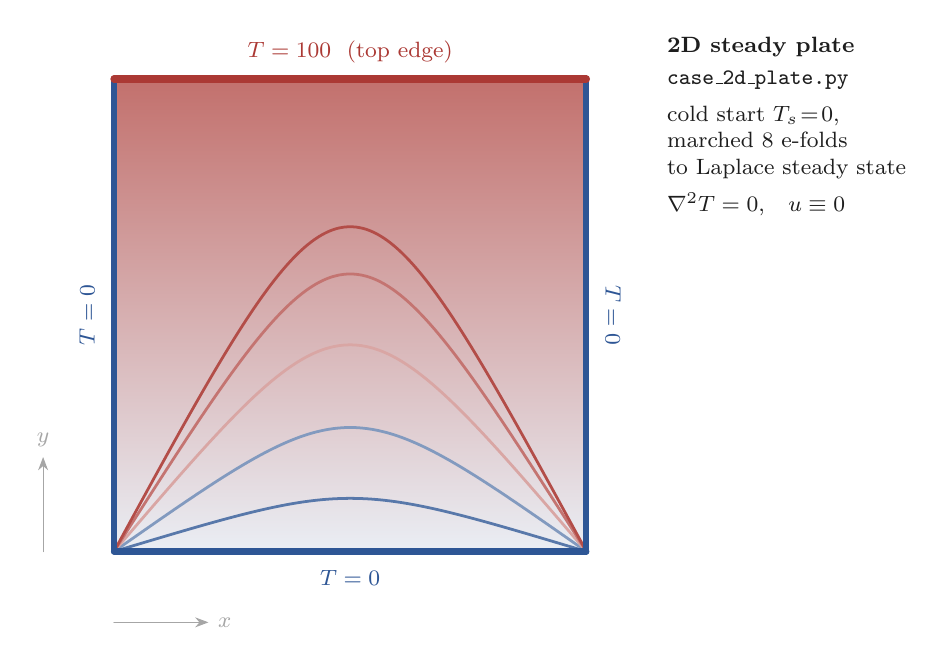
\begin{tikzpicture}[>=Stealth, font=\footnotesize, line cap=round]
  \def\S{6}  % side length in tikz units (represents L = 1)

  % interior temperature field: hot top -> cold bottom
  \shade[top color=hotc!72, bottom color=coldc!10] (0,0) rectangle (\S,\S);

  % steady isotherms: domes peaking under the hot top edge, pulled to 0 at the
  % cold side walls. Drawn cool (low) -> warm (high).
  \draw[coldc!80, line width=1pt] (0,0.0) .. controls (3,0.9) .. (\S,0.0);
  \draw[coldc!60, line width=1pt] (0,0.0) .. controls (3,2.1) .. (\S,0.0);
  \draw[hotc!45, line width=1pt]  (0,0.0) .. controls (3,3.5) .. (\S,0.0);
  \draw[hotc!70, line width=1pt]  (0,0.0) .. controls (3,4.7) .. (\S,0.0);
  \draw[hotc!90, line width=1pt]  (0,0.0) .. controls (3,5.5) .. (\S,0.0);

  % edges: top hot, the other three cold
  \draw[coldc, line width=2.2pt] (0,0) -- (\S,0);   % bottom
  \draw[coldc, line width=2.2pt] (0,0) -- (0,\S);   % left
  \draw[coldc, line width=2.2pt] (\S,0) -- (\S,\S); % right
  \draw[hotc,  line width=2.6pt] (0,\S) -- (\S,\S); % top

  % boundary-condition labels
  \node[hotc,  anchor=south] at (\S/2,\S+0.08) {$T=100$ \ (top edge)};
  \node[coldc, anchor=north] at (\S/2,-0.12) {$T=0$};
  \node[coldc, rotate=90, anchor=south] at (-0.12,\S/2) {$T=0$};
  \node[coldc, rotate=-90, anchor=south] at (\S+0.12,\S/2) {$T=0$};

  % axes
  \draw[->, gray!70] (0,-0.9) -- (1.2,-0.9) node[right]{$x$};
  \draw[->, gray!70] (-0.9,0) -- (-0.9,1.2) node[above]{$y$};

  % annotation
  \node[inkc, anchor=west, align=left] at (\S+0.9,\S-0.6)
    {\textbf{2D steady plate}\\[2pt]
     \texttt{case\_2d\_plate.py}\\[4pt]
     cold start $T_s\!=\!0$,\\
     marched $8$ e-folds\\
     to Laplace steady state\\[4pt]
     $\nabla^2 T = 0$,\quad $u\equiv 0$};
\end{tikzpicture}
\end{document}
